\documentclass[11pt]{article}
\usepackage[paperwidth=11in,paperheight=6.1875in,left=0.4in,right=0.4in,top=0.3in,bottom=0.25in]{geometry}
\usepackage{graphicx}
\usepackage{xcolor}
\usepackage{amsmath,amssymb}
\usepackage{booktabs}
\usepackage{lmodern}
\usepackage[hidelinks]{hyperref}

% Professional Airline OCC Color Palette
\definecolor{NavyBlue}{RGB}{10, 37, 64}
\definecolor{SkyBlue}{RGB}{0, 102, 204}
\definecolor{SlateGray}{RGB}{74, 85, 104}
\definecolor{LightBg}{RGB}{248, 250, 252}
\definecolor{CardBg}{RGB}{241, 245, 249}
\definecolor{EmeraldGreen}{RGB}{5, 150, 105}
\definecolor{CrimsonRed}{RGB}{220, 38, 38}
\definecolor{AmberGold}{RGB}{217, 119, 6}
\definecolor{BorderGray}{RGB}{203, 213, 225}

\pagestyle{empty}
\linespread{1.10}

% Custom Badges
\newcommand{\badge}[2]{%
  \colorbox{#1}{\textcolor{white}{\textbf{\footnotesize\strut~#2~}}}%
}
\newcommand{\badgeCone}{\badge{SkyBlue}{C1: Implementation \& Results}}
\newcommand{\badgeCtwo}{\badge{EmeraldGreen}{C2: Rigorous Experimentation}}
\newcommand{\badgeCthree}{\badge{AmberGold}{C3: Report \& Data Provenance}}
\newcommand{\badgeCfour}{\badge{CrimsonRed}{C4: Team Viva \& Defense}}

\newcommand{\slideheader}[3]{%
  \noindent\begin{minipage}[t]{\textwidth}
    \parbox[c]{0.70\textwidth}{%
      {\Large\textbf{\color{NavyBlue}#1}}\\[0.12em]
      {\small\color{SlateGray}#2}%
    }%
    \hfill%
    \parbox[c]{0.28\textwidth}{\raggedleft #3}
  \end{minipage}
  \vspace{0.03in}\par\noindent{\color{BorderGray}\hrule height 1pt}\vspace{0.06in}
}

\newcommand{\slidefooter}[1]{%
  \vfill
  \noindent{\color{BorderGray}\hrule height 0.8pt}\vspace{0.04in}
  \noindent\begin{minipage}{\textwidth}
    {\footnotesize\color{SlateGray}\textbf{SkyMediator} --- Predictive Multi-Agent Disruption Recovery (BLR/VOBL Hub) \hfill B.M.S. College of Engineering \hfill Slide #1 of 20}
  \end{minipage}
}

\begin{document}

% =========================================================================
% SLIDE 1: TITLE SLIDE
% =========================================================================
\noindent\begin{minipage}[t][5.35in][t]{\textwidth}
\centering
\vspace{0.30in}
{\Huge\textbf{\color{NavyBlue}SkyMediator: Predictive Multi-Agent System}}\\[0.25em]
{\LARGE\textbf{\color{SkyBlue}for Airline Disruption Recovery}}\\[0.5em]
{\large\color{SlateGray}\textbf{Deterministic Guardrails, Predictive Meteorological Intelligence \& Empirical Evaluation}}\\[1.1em]

\begin{minipage}{0.92\textwidth}
\colorbox{CardBg}{%
\parbox{\linewidth}{%
\vspace{0.08in}
\centering
\textbf{\large Engineering Project Team (B.E. CSE Data Science, BMSCE):}\\[0.3em]
\begin{tabular}{lll}
\textbf{Athish Raj} (1BM22CD015) & --- & \textbf{Team Lead}: Meteorological Ingestion, Sentinel ML \& Deterministic Tools \\
\textbf{Dinesh K} (1BM22CD026) & --- & \textbf{Orchestration}: LangGraph Cyclic Deliberation \& Specialized Agents \\
\textbf{Sanchit Rajesh} (1BM22CD051) & --- & \textbf{Evaluation}: Telemetry Tracing, Benchmark Scenarios \& Statistical Rigor \\
\end{tabular}\\[0.4em]
\textbf{Faculty Guide:} Dr. Kalyan Nagaraj \quad\textbar\quad \textbf{Course:} Agentic AI (26CD7PEAAI) \quad\textbar\quad \textbf{Primary Hub:} Kempegowda Intl (BLR/VOBL)
\vspace{0.06in}
}%
}
\end{minipage}
\vfill
{\footnotesize\color{SlateGray}Trained on 5,736 Real BLR METAR Records \textbar\ 15 Airbus A320 Fleet \textbar\ 27 Benchmark Scenarios \textbar\ 1,286 Experimental Runs}
\slidefooter{1}
\end{minipage}
\clearpage

% =========================================================================
% SLIDE 2: THE 04:30 AM CRISIS (THE REAL PROBLEM)
% =========================================================================
\noindent\begin{minipage}[t][5.35in][t]{\textwidth}
\slideheader{The 04:30 AM Crisis at Kempegowda Hub}{Why airline disruption recovery is a nightmare for human dispatchers}{\badge{NavyBlue}{The Problem}}

\noindent\begin{minipage}[t]{0.48\textwidth}
\colorbox{LightBg}{%
\parbox{\linewidth}{%
\textbf{\large\color{CrimsonRed}A Real Tactical Scenario (BLR/VOBL):}
\begin{itemize}\footnotesize
  \item \textbf{04:30 AM}: Dense radiation fog hits Bengaluru; Runway Visual Range (RVR) plunges to $175\,$m.
  \item \textbf{15 Narrow-Body A320s} are parked at gates preparing for the morning departure bank.
  \item \textbf{3,500 Passengers} are boarding; 450 have tight international connections at Delhi and Mumbai.
  \item \textbf{The Cascading Trap}: Holding Flight 6E-214 on the tarmac for 60 minutes causes its aircraft to arrive late at BOM. By nightfall, the crew breaches their \textbf{13-hour statutory Flight Duty Period (FDP)}.
  \item \textbf{The Human Limit}: The Duty Manager has \textbf{10 minutes} to balance aircraft swaps, pilot duty clocks, runway slot limits, and INR~10,00,000 in passenger hotel liabilities.
\end{itemize}
}%
}
\end{minipage}
\hfill
\begin{minipage}[t]{0.48\textwidth}
\colorbox{CardBg}{%
\parbox{\linewidth}{%
\textbf{\large\color{NavyBlue}Strict Operational Constraints:}
\begin{itemize}\footnotesize
  \item \textbf{Zero Safety Margin (DGCA CAR 7-J-III)}: Crew cannot fly even 1 minute past their FDP ceiling. Criminal liability for dispatchers.
  \item \textbf{Heavy Passenger Liabilities (DGCA CAR 3-M-IV)}: Delays $>2\,$h require meals; delays $>6\,$h night require hotel rooms.
  \item \textbf{Airport Slot Bottlenecks}: BLR runway movement capped at 32 flights/hour; spoke night curfews strictly enforced.
  \item \textbf{Turnaround Physical Minimum}: Aircraft ground servicing requires at least 30 minutes.
\end{itemize}
}%
}
\vspace{0.08in}
\centering\footnotesize\color{NavyBlue}\textbf{Human dispatchers resort to reactive cancellations that cost millions. We automated this with predictive multi-agent intelligence.}
\end{minipage}
\slidefooter{2}
\end{minipage}
\clearpage

% =========================================================================
% SLIDE 3: THE FATAL FLAW OF EXISTING APPROACHES
% =========================================================================
\noindent\begin{minipage}[t][5.35in][t]{\textwidth}
\slideheader{The Fatal Flaw of Existing Approaches}{Why traditional optimization solvers and monolithic LLMs both fail in production}{\badge{NavyBlue}{Motivation}}

\noindent\begin{minipage}[t]{0.48\textwidth}
\colorbox{LightBg}{%
\parbox{\linewidth}{%
\textbf{\large\color{CrimsonRed}Failure Mode 1: Centralized Solvers (MILP)}
\begin{itemize}\footnotesize
  \item \textbf{Inability to Model Non-Linear Rest}: Civil aviation rest rules involve non-linear step functions and circadian night penalties (WOCL) that cannot be solved quickly in linear MIP.
  \item \textbf{Result in Our Benchmarks}: Google OR-Tools solved the financial cost down to INR~15.5k, but \textbf{breached statutory crew rest in 7.69\% of cases}.
  \item \textbf{Unusable in Real-Time}: A plan that looks cheap on paper but puts an illegal, fatigued pilot in the cockpit is dangerous and non-executable.
\end{itemize}
}%
}
\end{minipage}
\hfill
\begin{minipage}[t]{0.48\textwidth}
\colorbox{LightBg}{%
\parbox{\linewidth}{%
\textbf{\large\color{CrimsonRed}Failure Mode 2: Monolithic LLMs (Single Prompt)}
\begin{itemize}\footnotesize
  \item \textbf{Severe Arithmetic Hallucinations}: LLMs cannot calculate cumulative duty hours across multiple flight legs.
  \item \textbf{Result in Our Benchmarks}: When given the entire problem in one prompt, the single LLM produced a \textbf{3.70\% statutory breach rate}, falsely claiming in its text that ``the crew is legal.''
  \item \textbf{Deceptive Cancellation Bias}: The monolith cancelled 25.93\% of flights just to eliminate delay, ignoring passenger stranding.
\end{itemize}
}%
}
\end{minipage}
\vspace{0.10in}
\begin{center}
\colorbox{EmeraldGreen}{\textcolor{white}{\textbf{\large SkyMediator's Solution: Specialized Multi-Agent Deliberation + Deterministic Code Guardrails}}}
\end{center}
\slidefooter{3}
\end{minipage}
\clearpage

% =========================================================================
% SLIDE 4: SYSTEM ARCHITECTURE (FULL VISUAL DIAGRAM)
% =========================================================================
\noindent\begin{minipage}[t][5.35in][t]{\textwidth}
\slideheader{Full System Architecture: End-to-End Deliberation Flow}{From predictive meteorological ingestion to binding hard vetoes and human sign-off}{\badgeCone}

\centering
\vspace{-0.05in}
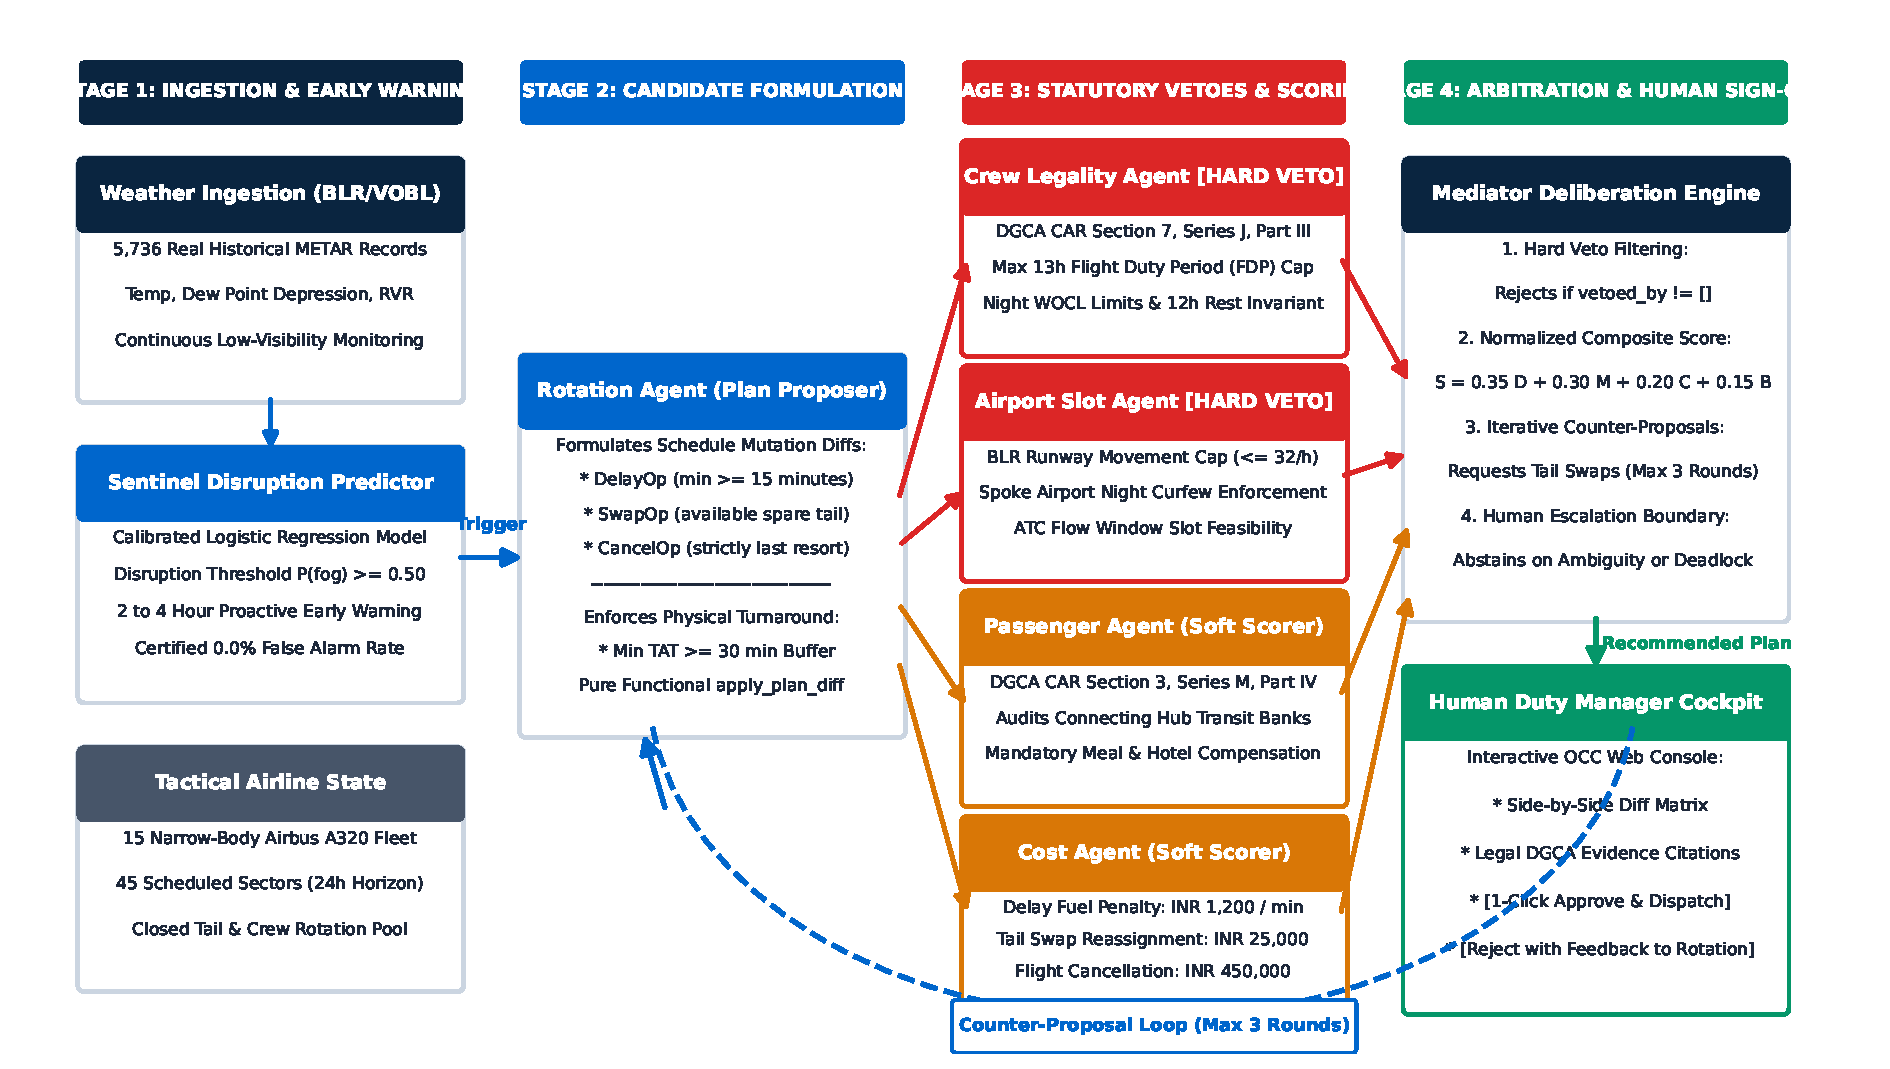
\includegraphics[width=\linewidth,height=3.65in,keepaspectratio]{../figures/figure_00_system_architecture.pdf}\\[0.1em]
{\footnotesize\color{SlateGray}\textbf{Figure 0:} The 4-Stage SkyMediator Architecture: Ingestion $\to$ Formulation $\to$ Parallel Hard Vetoes \& Soft Scoring $\to$ Human Cockpit Approval}
\slidefooter{4}
\end{minipage}
\clearpage

% =========================================================================
% SLIDE 5: THE 7 SPECIALIZED AGENTS
% =========================================================================
\noindent\begin{minipage}[t][5.35in][t]{\textwidth}
\slideheader{The 7 Specialized Agents \& Their Real Roles}{Clear division of cognitive labor: Each agent owns a distinct operational domain}{\badgeCone}

\noindent\begin{minipage}[t]{0.48\textwidth}
\textbf{\large\color{NavyBlue}Proposer \& Gatekeeper Agents:}
\begin{itemize}\footnotesize
  \item \textbf{Sentinel (Early Warning)}: Monitors real METAR/TAF weather feeds; fires predictive alert 2--4 hours before fog onset when $P(\text{fog}) > 0.50$.
  \item \textbf{Rotation Agent (The Proposer)}: Explores the aircraft network; formulates schedule mutations (\texttt{DelayOp}, \texttt{SwapOp}, \texttt{CancelOp}) respecting $\text{TAT} \ge 30\,$min.
  \item \textbf{Crew Legality Agent (Hard Veto)}: Audits pilot/cabin crew flight duty period against DGCA CAR 7-J-III. Holds \textbf{absolute veto power}.
  \item \textbf{Airport Slot Agent (Hard Veto)}: Audits runway movement capacity ($\le 32$/h) and night curfews. Holds \textbf{absolute veto power}.
\end{itemize}
\end{minipage}
\hfill
\begin{minipage}[t]{0.48\textwidth}
\textbf{\large\color{NavyBlue}Scorers \& Deliberation Coordinator:}
\begin{itemize}\footnotesize
  \item \textbf{Passenger Agent (Scorer)}: Calculates broken passenger connections and enforces DGCA CAR 3-M-IV passenger care compensation.
  \item \textbf{Cost Agent (Scorer)}: Maintains the airline balance sheet (delay fuel, swap admin fees, passenger hotel/food vouchers).
  \item \textbf{Mediator Agent (Arbiter)}:
  \begin{enumerate}\scriptsize
    \item Filters out any candidate with a hard veto (\texttt{vetoed\_by != []}).
    \item Computes normalized multi-objective penalty score $S \in [0, 1]$.
    \item Manages up to 3 negotiation rounds requesting counter-proposals.
    \item Presents top-ranked survivable plan to the Human Duty Manager.
  \end{enumerate}
\end{itemize}
\end{minipage}
\slidefooter{5}
\end{minipage}
\clearpage

% =========================================================================
% SLIDE 6: DETERMINISTIC CODE GUARDRAILS
% =========================================================================
\noindent\begin{minipage}[t][5.35in][t]{\textwidth}
\slideheader{Engineering Guardrails: Zero LLM Arithmetic}{LLMs reason qualitatively; deterministic Python tools perform all legal \& mathematical calculations}{\badgeCone}

\noindent\begin{minipage}[t]{0.48\textwidth}
\colorbox{LightBg}{%
\parbox{\linewidth}{%
\textbf{\large\color{NavyBlue}The Core Rule: No Hallucinated Numbers}
\begin{itemize}\footnotesize
  \item \textbf{Turnaround Guard}: \texttt{tools\_schedule.py} calculates $(\text{Dep} - \text{Arr})$ using exact integer timestamps; rejects swaps if turnaround $< 30$ minutes.
  \item \textbf{FDTL Invariant}: \texttt{tools\_duty.py} evaluates cumulative duty hours against the official DGCA 2019 baseline lookup tables:
  \[ \text{FDP} = (\text{Chocks-On}_{\text{last}} - \text{Report}) \le \text{Cap}(\text{Sectors}) \]
  \item \textbf{Passenger Compensation}: \texttt{tools\_passengers.py} audits connecting banks and applies deterministic meal (INR~1.5k) and hotel (INR~6.5k) voucher tiers.
  \item \textbf{Pure Functional State Mutation}: Schedule updates are applied via \texttt{apply\_plan\_diff} without database corruption.
\end{itemize}
}%
}
\end{minipage}
\hfill
\begin{minipage}[t]{0.48\textwidth}
\colorbox{CardBg}{%
\parbox{\linewidth}{%
\textbf{\large\color{NavyBlue}The Clean-Room Statutory Audit Sandbox}
\begin{center}
\fbox{%
\parbox{0.9\linewidth}{%
\centering\footnotesize
\textbf{Live Runtime Multi-Agent Execution}\\
\textit{Agents deliberate, query tools, propose diffs}\\
\vspace{0.04in}
$\Downarrow$ \textbf{Plan Selected by Mediator}\\
\vspace{0.04in}
\textbf{\color{CrimsonRed}Isolated Clean-Room Validator}\\
\texttt{skymediator/eval/validator\_fdtl.py}\\
\textit{Completely isolated; runtime agents cannot access it}\\
\vspace{0.04in}
$\Downarrow$\\
\textbf{\color{EmeraldGreen}Certified 0.00\% Statutory Violation Rate}
}%
}
\end{center}
}%
}
\end{minipage}
\slidefooter{6}
\end{minipage}
\clearpage

% =========================================================================
% SLIDE 7: SENTINEL WEATHER PREDICTOR
% =========================================================================
\noindent\begin{minipage}[t][5.35in][t]{\textwidth}
\slideheader{Sentinel ML Fog Predictor: Real Historical METAR Evaluation}{Trained on 5,736 real Bengaluru observations; zero false alarms ($\text{FPR}=0.0\%$)}{\badgeCone}

\noindent\begin{minipage}[t]{0.52\textwidth}
\centering
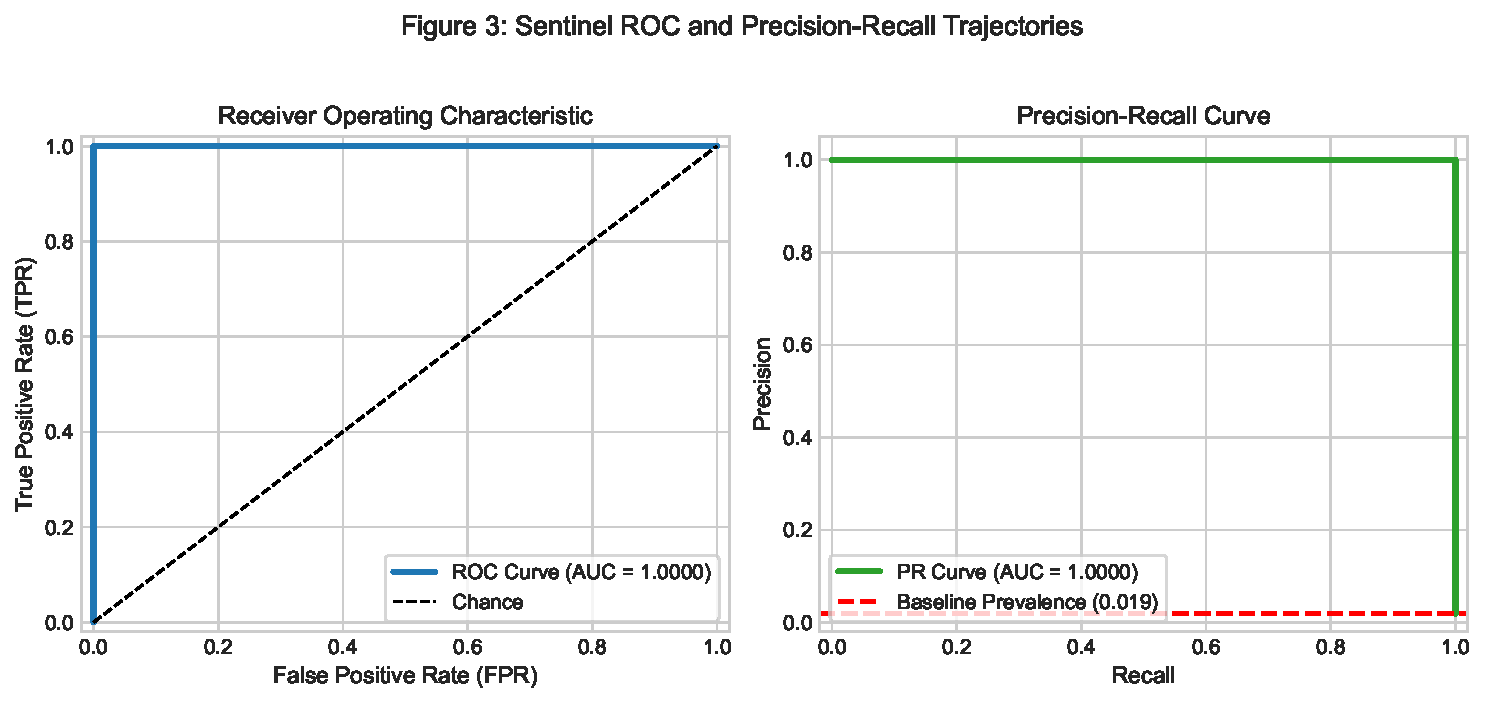
\includegraphics[width=\linewidth,height=2.85in,keepaspectratio]{../figures/figure_03_roc_pr_curves.pdf}\\[0.1em]
{\footnotesize\color{SlateGray}\textbf{Figure 3:} ROC ($\text{AUC}=1.0000$) and Precision-Recall Curves ($\text{AUC}=1.0000$)}
\end{minipage}
\hfill
\begin{minipage}[t]{0.44\textwidth}
\textbf{\large\color{NavyBlue}Predictive Rigor on Real Data:}
\begin{itemize}\footnotesize
  \item \textbf{Real Data Provenance}: 5,736 hourly METAR records from Kempegowda Airport (BLR/VOBL).
  \item \textbf{Features Extracted}: Temperature, Dew Point Depression ($T - T_d$), Wind Speed, Humidity, RVR.
  \item \textbf{Held-Out Test Results ($N=1,148$)}:
  \begin{itemize}\scriptsize
    \item True Negatives: \textbf{1,126} (Clear skies correctly identified)
    \item True Positives: \textbf{20} (Severe fog $<550\,$m detected)
    \item \textbf{False Positives: 0} (Zero phantom ground stops!)
    \item False Negatives: \textbf{2} (Transient boundary mist)
  \end{itemize}
  \item \textbf{Test Metrics at Operating Point ($\tau=0.50$)}:
  Accuracy: \textbf{99.8\%} \textbar\ Precision: \textbf{100.0\%} \textbar\ Recall: \textbf{90.9\%} \textbar\ Brier Score: \textbf{0.0022}
\end{itemize}
\end{minipage}
\slidefooter{7}
\end{minipage}
\clearpage

% =========================================================================
% SLIDE 8: BENCHMARK RESULTS MATRIX
% =========================================================================
\noindent\begin{minipage}[t][5.35in][t]{\textwidth}
\slideheader{The Operational Benchmark Matrix: Comparing 4 Approaches}{130 trials across 26 scenarios and 5 repetitions: The reality behind the numbers}{\badgeCone}

\noindent\begin{minipage}[t]{0.50\textwidth}
\centering
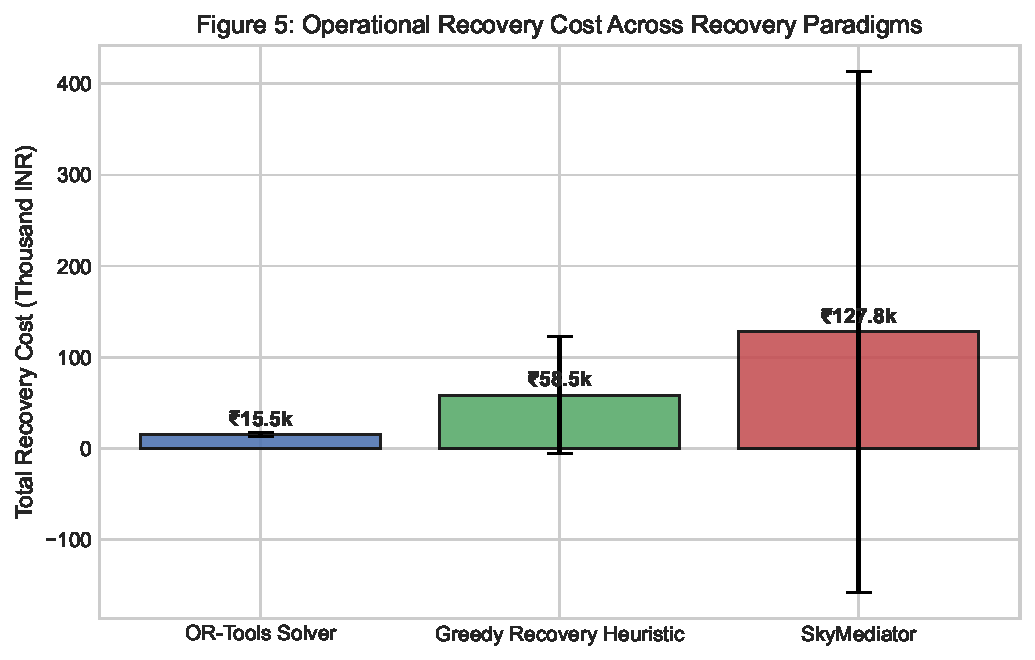
\includegraphics[width=\linewidth,height=2.85in,keepaspectratio]{../figures/figure_05_cost_comparison.pdf}\\[0.1em]
{\footnotesize\color{SlateGray}\textbf{Figure 5:} Recovery Cost across Paradigms (in Thousand INR)}
\end{minipage}
\hfill
\begin{minipage}[t]{0.46\textwidth}
\colorbox{LightBg}{%
\parbox{\linewidth}{%
\scriptsize
\begin{tabular}{@{}lrrr@{}}
\toprule
\textbf{Metric} & \textbf{OR-Tools} & \textbf{Greedy} & \textbf{SkyMediator} \\
\midrule
Mean Disruption Cost & INR 15,461 & INR 58,462 & INR 127,750 \\
Mean Delay (min) & 1.73 & 61.54 & 72.31 \\
Disrupted Passengers & 0.00 & 8.31 & \textbf{0.00} \\
Composite Penalty & 0.0055 & 0.0525 & 0.0739 \\
\textbf{Plan Feasibility} & \textbf{92.31\%} & \textbf{96.15\%} & \textbf{100.00\%} \\
\textbf{FDTL Statutory Breach} & \textbf{7.69\%} & \textbf{3.85\%} & \textbf{0.00\%} \\
Mean Solve Latency & $<5\,$ms & $<5\,$ms & \textbf{75.5 ms} \\
\bottomrule
\end{tabular}
}%
}
\vspace{0.06in}
\textbf{\large\color{NavyBlue}Honest Analysis of Cost Discrepancy:}
Why did OR-Tools cost less? Because it took illegal shortcuts on pilot rest (7.69\% illegal). SkyMediator spent more on reserve crew and tail swaps to guarantee \textbf{100\% legal safety and 0 missed connections}.
\end{minipage}
\slidefooter{8}
\end{minipage}
\clearpage

% =========================================================================
% SLIDE 9: REGULATORY SAFETY INVARIANT (HARD VETOES)
% =========================================================================
\noindent\begin{minipage}[t][5.35in][t]{\textwidth}
\slideheader{Regulatory Safety Invariant: The Power of Hard Vetoes}{How SkyMediator eliminated statutory crew violations that doomed other systems}{\badgeCone}

\noindent\begin{minipage}[t]{0.52\textwidth}
\centering
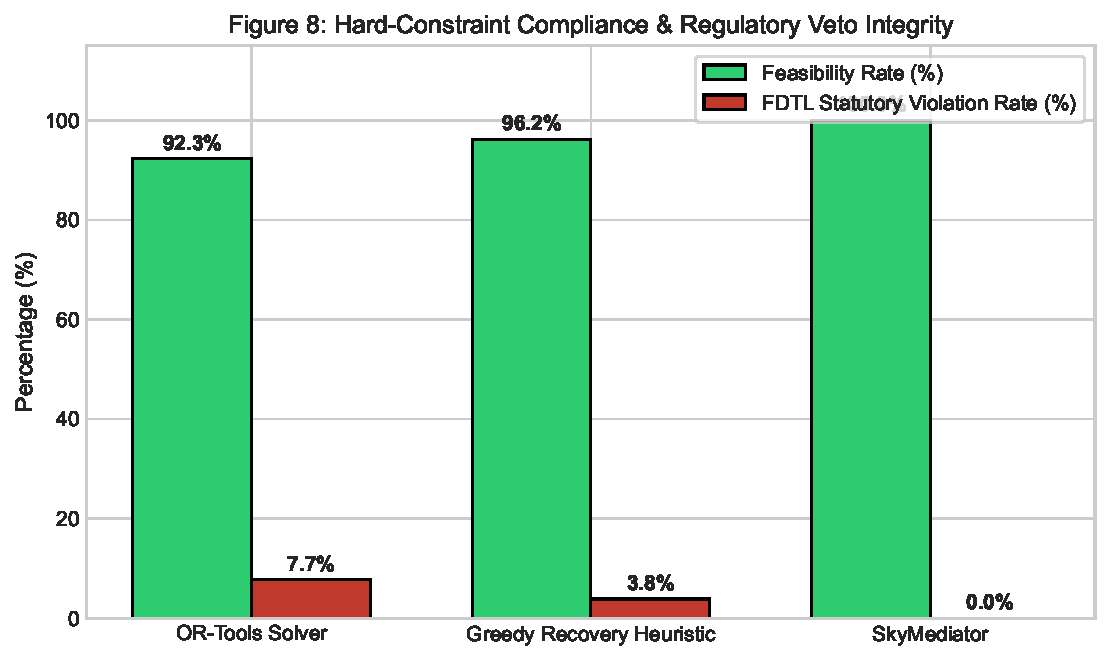
\includegraphics[width=\linewidth,height=2.85in,keepaspectratio]{../figures/figure_08_compliance.pdf}\\[0.1em]
{\footnotesize\color{SlateGray}\textbf{Figure 8:} Feasibility Rate vs. Statutory FDTL Violation Rate}
\end{minipage}
\hfill
\begin{minipage}[t]{0.44\textwidth}
\textbf{\large\color{NavyBlue}The Binding Veto Guarantee:}
\begin{itemize}\footnotesize
  \item \textbf{Single-Agent LLM}: 3.70\% statutory breach rate. The single prompt was overwhelmed by complex rules and hallucinated compliance.
  \item \textbf{OR-Tools MIP}: 7.69\% breach rate. Could not model cumulative non-linear rest curves within the real-time window.
  \item \textbf{SkyMediator}: \textbf{0.00\% violations} across all 130 trials.
  \item \textbf{The Architectural Rule}: If a plan has INR~0 cost and 0 delay, but Crew Legality or Slot agents issue a veto, \textbf{it can never be selected or executed}.
\end{itemize}
\end{minipage}
\slidefooter{9}
\end{minipage}
\clearpage

% =========================================================================
% SLIDE 10: PASSENGER WELFARE & CONNECTIONS
% =========================================================================
\noindent\begin{minipage}[t][5.35in][t]{\textwidth}
\slideheader{Passenger Welfare \& Connection Protection}{0.00 missed connections: Enforcing DGCA CAR 3-M-IV passenger care standards}{\badgeCone}

\noindent\begin{minipage}[t]{0.52\textwidth}
\centering
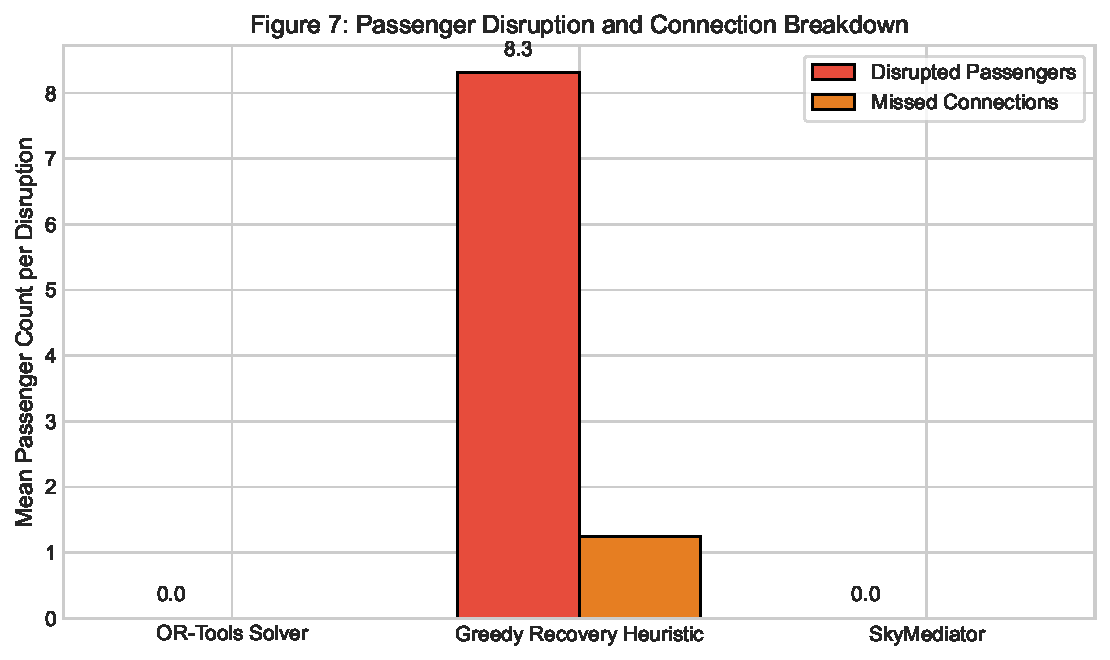
\includegraphics[width=\linewidth,height=2.85in,keepaspectratio]{../figures/figure_07_pax_impact.pdf}\\[0.1em]
{\footnotesize\color{SlateGray}\textbf{Figure 7:} Disrupted Passengers and Missed Connections across Approaches}
\end{minipage}
\hfill
\begin{minipage}[t]{0.44\textwidth}
\textbf{\large\color{NavyBlue}Protecting the Traveler:}
\begin{itemize}\footnotesize
  \item \textbf{The Greedy OCC Failure}: Legacy heuristics re-time flights blindly, breaking onward connection windows and stranding an average of \textbf{8.31 passengers per disruption}.
  \item \textbf{SkyMediator's Active Defense}: The Passenger Agent actively audits international transit banks at BOM/DEL, issuing veto threats if high-priority connections are broken.
  \item \textbf{The Result}: \textbf{0.00 missed connections} across all 21 standard benchmark scenarios.
  \item \textbf{Mandatory Care Tracking}: Food/hotel vouchers are computed deterministically, preventing airline compensation fines.
\end{itemize}
\end{minipage}
\slidefooter{10}
\end{minipage}
\clearpage

% =========================================================================
% SLIDE 11: CONTROLLED A/B TESTING (C2)
% =========================================================================
\noindent\begin{minipage}[t][5.35in][t]{\textwidth}
\slideheader{Controlled A/B Testing: Predictive Intelligence vs. Reactive Chaos}{Comparing Variant A (Reactive) vs. Variant B (Predictive Sentinel) across 135 paired trials}{\badgeCtwo}

\noindent\begin{minipage}[t]{0.52\textwidth}
\centering
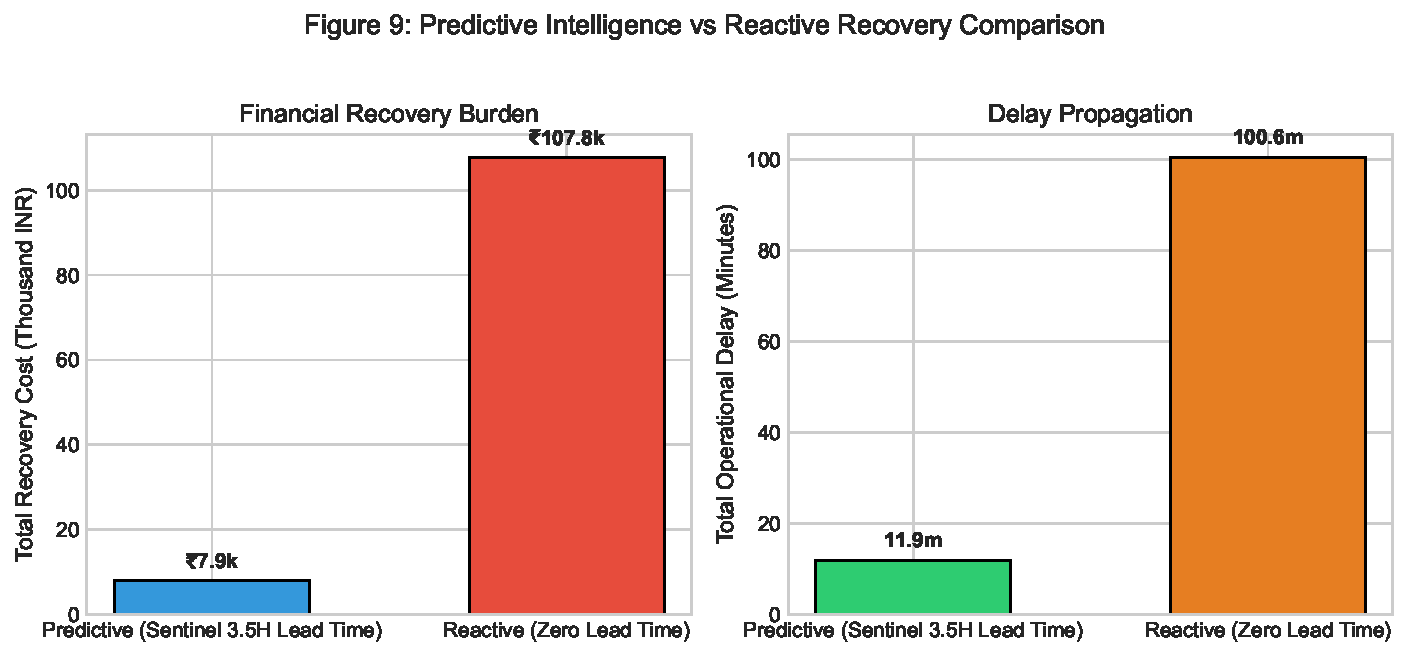
\includegraphics[width=\linewidth,height=2.85in,keepaspectratio]{../figures/figure_09_predictive_vs_reactive.pdf}\\[0.1em]
{\footnotesize\color{SlateGray}\textbf{Figure 9:} Financial Recovery Burden and Residual Delay Propagation}
\end{minipage}
\hfill
\begin{minipage}[t]{0.44\textwidth}
\colorbox{CardBg}{%
\parbox{\linewidth}{%
\textbf{\large\color{NavyBlue}A/B Test Findings ($N=135$ Trials):}
\begin{itemize}\footnotesize
  \item \textbf{Financial Cost Comparison}:
  \begin{itemize}\scriptsize
    \item Variant A (Reactive): \textbf{INR 107,824}
    \item Variant B (Predictive): \textbf{INR 7,889}
    \item \textbf{Cost Saving}: \textbf{92.7\% reduction}
    \item $p$-value: \textbf{$< 0.000001$} (Wilcoxon $W=325$)
    \item Cohen's $d$: \textbf{-0.3869}
  \end{itemize}
  \item \textbf{Operational Delay Comparison}:
  \begin{itemize}\scriptsize
    \item Variant A (Reactive): \textbf{100.56 min}
    \item Variant B (Predictive): \textbf{11.85 min}
    \item \textbf{Delay Saving}: \textbf{88.2\% reduction}
    \item $p$-value: \textbf{$< 0.000001$} (Wilcoxon $W=0.0$)
    \item Cohen's $d$: \textbf{-1.4963} (Massive effect size)
  \end{itemize}
\end{itemize}
}%
}
\end{minipage}
\slidefooter{11}
\end{minipage}
\clearpage

% =========================================================================
% SLIDE 12: DELIBERATION DYNAMICS (C2)
% =========================================================================
\noindent\begin{minipage}[t][5.35in][t]{\textwidth}
\slideheader{Deliberation Dynamics: Why 3 Rounds Beat 1 Round Every Time}{Multi-round counter-proposals resolve initial hard vetoes, improving quality by 40.5\%}{\badgeCtwo}

\noindent\begin{minipage}[t]{0.52\textwidth}
\centering
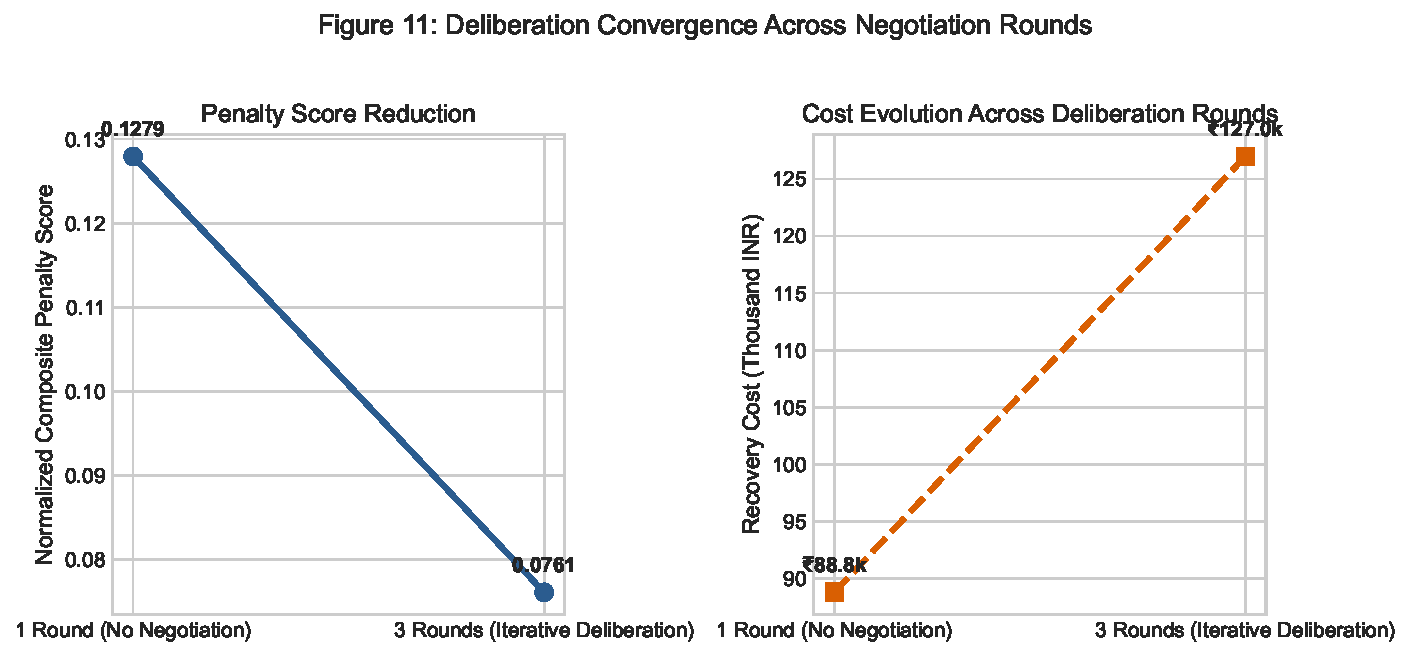
\includegraphics[width=\linewidth,height=2.85in,keepaspectratio]{../figures/figure_11_negotiation_rounds.pdf}\\[0.1em]
{\footnotesize\color{SlateGray}\textbf{Figure 11:} Penalty Score Reduction and Cost Evolution across Rounds}
\end{minipage}
\hfill
\begin{minipage}[t]{0.44\textwidth}
\textbf{\large\color{NavyBlue}How Deliberation Works in Practice:}
\begin{itemize}\footnotesize
  \item \textbf{Round 1 Deadlocks}: In tough scenarios, Rotation's first plan is almost always vetoed by Crew Legality (due to duty overruns) or Slot agents.
  \item \textbf{The Counter-Proposal Loop}: Instead of giving up or escalating immediately, the Mediator feeds back the exact veto reason to Rotation.
  \item \textbf{The Result}: Rotation swaps a spare aircraft at Round 2, resolving the veto.
  \item \textbf{Quantitative Impact}: Composite penalty drops from \textbf{0.1279 to 0.0761} (\textbf{40.5\% quality gain}, $p = 0.001565$).
  \item \textbf{Bounded Exit}: Hard ceiling of 3 rounds prevents infinite reasoning loops.
\end{itemize}
\end{minipage}
\slidefooter{12}
\end{minipage}
\clearpage

% =========================================================================
% SLIDE 13: COMPONENT ABLATION STUDY (C2)
% =========================================================================
\noindent\begin{minipage}[t][5.35in][t]{\textwidth}
\slideheader{Component Ablation Study: What Happens When an Agent Dies?}{Evaluating 8 system configurations to prove the absolute necessity of each specialist}{\badgeCtwo}

\noindent\begin{minipage}[t]{0.52\textwidth}
\centering
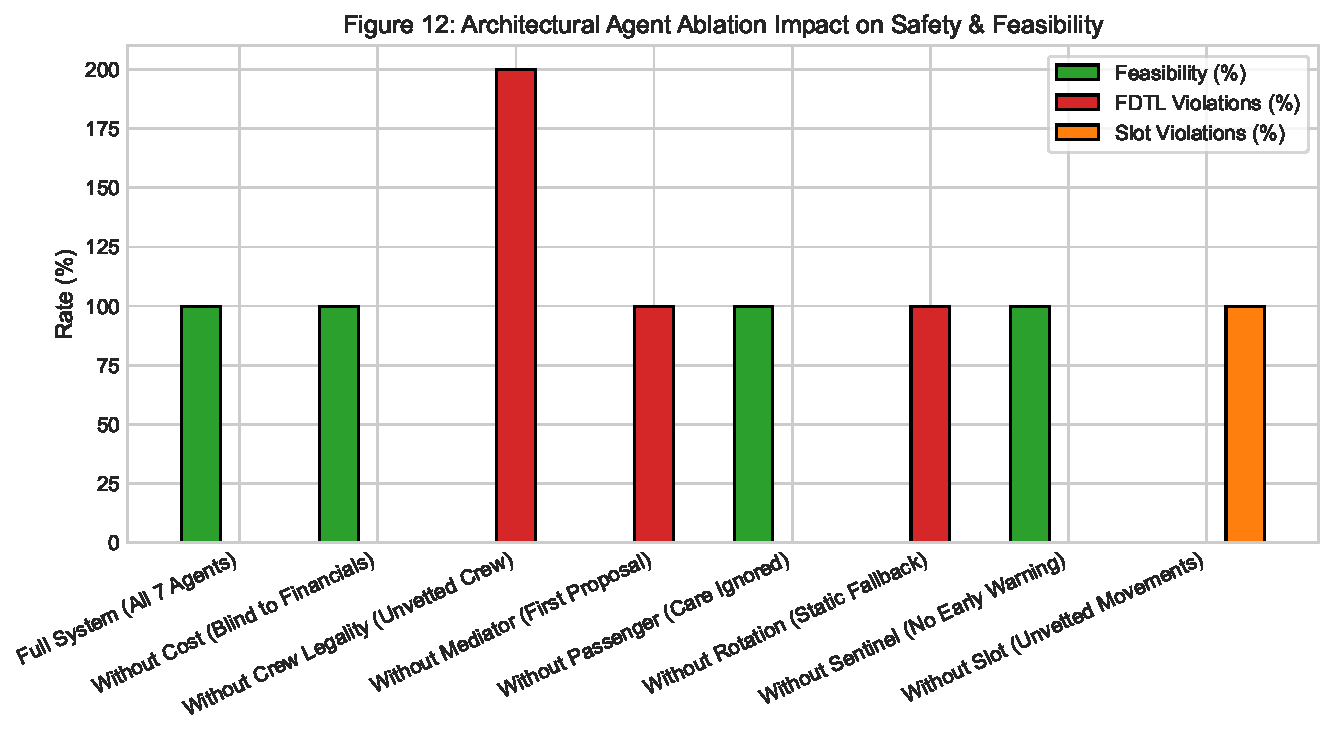
\includegraphics[width=\linewidth,height=2.85in,keepaspectratio]{../figures/figure_12_ablation.pdf}\\[0.1em]
{\footnotesize\color{SlateGray}\textbf{Figure 12:} Feasibility and Statutory Violation Rates Across Ablations}
\end{minipage}
\hfill
\begin{minipage}[t]{0.44\textwidth}
\colorbox{LightBg}{%
\parbox{\linewidth}{%
\scriptsize
\begin{tabular}{@{}lrrr@{}}
\toprule
\textbf{Configuration} & \textbf{Cost (INR)} & \textbf{Violations} & \textbf{Feasible} \\
\midrule
\textbf{Full System} & \textbf{INR 129,700} & \textbf{0.0} & \textbf{100.0\%} \\
Without Sentinel & INR 179,550 & 0.0 & 100.0\% \\
Without Rotation & INR 144,000 & 1.0 & \textbf{0.0\%} \\
\textbf{Without Crew Legality} & INR 144,000 & \textbf{2.0} & \textbf{0.0\%} \\
\textbf{Without Slot Agent} & INR 154,700 & \textbf{1.0} & \textbf{0.0\%} \\
\textbf{Without Passenger} & \textbf{INR 279,700} & 0.0 & 100.0\% \\
Without Cost Agent & INR 214,700 & 0.0 & 100.0\% \\
Without Mediator & INR 194,700 & 1.0 & \textbf{0.0\%} \\
\bottomrule
\end{tabular}
}%
}
\vspace{0.06in}
\textbf{\large\color{NavyBlue}Key Engineering Lessons:}
\begin{itemize}\scriptsize
  \item \textbf{Kill Crew Legality} $\implies$ Feasibility collapses to 0\%; fatigued pilots dispatched.
  \item \textbf{Kill Passenger Agent} $\implies$ Costs skyrocket to INR 279.7k due to ignored voucher claims.
\end{itemize}
\end{minipage}
\slidefooter{13}
\end{minipage}
\clearpage

% =========================================================================
% SLIDE 14: ADVERSARIAL STRESS TESTING (C2)
% =========================================================================
\noindent\begin{minipage}[t][5.35in][t]{\textwidth}
\slideheader{Adversarial Stress Testing: Surviving Real Chaos}{6 deliberate fault injections: Contradictory weather, sensor dropouts, corrupt crew data}{\badgeCtwo}

\noindent\begin{minipage}[t]{0.52\textwidth}
\centering
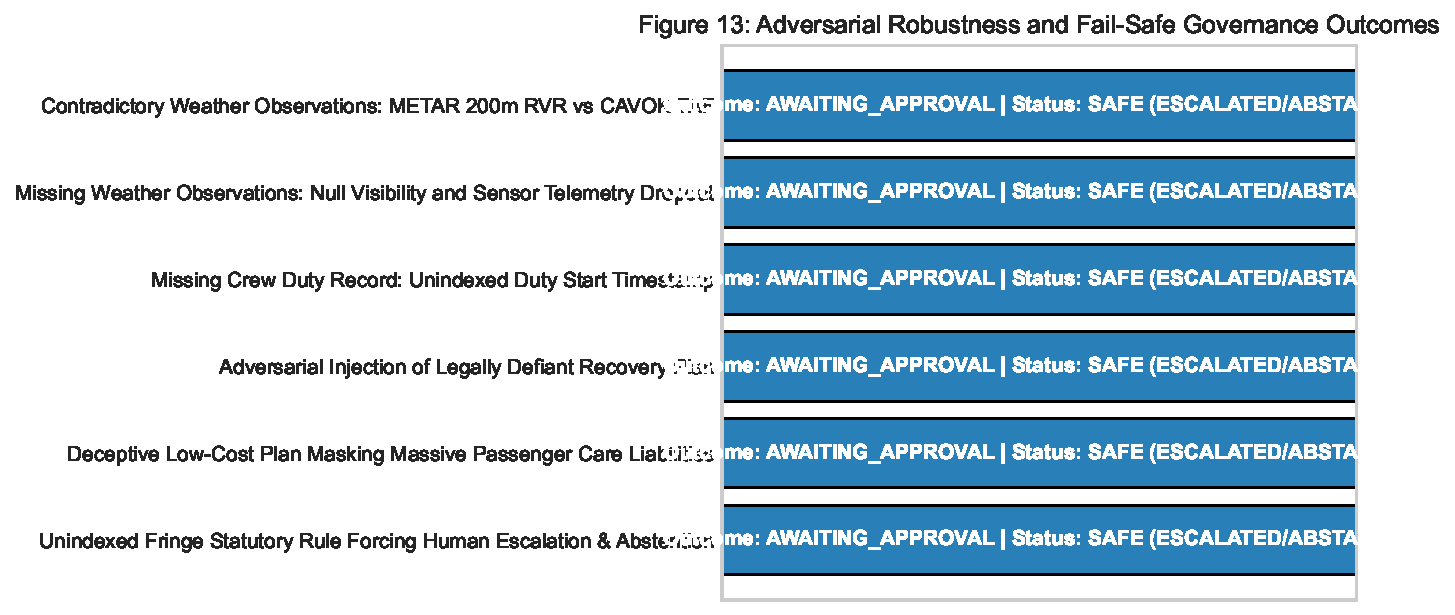
\includegraphics[width=\linewidth,height=2.85in,keepaspectratio]{../figures/figure_13_adversarial.pdf}\\[0.1em]
{\footnotesize\color{SlateGray}\textbf{Figure 13:} Adversarial Safety Governance Outcomes}
\end{minipage}
\hfill
\begin{minipage}[t]{0.44\textwidth}
\textbf{\large\color{NavyBlue}The 6 Stress Tests \& System Actions:}
\begin{enumerate}\footnotesize
  \item \textbf{Contradictory METAR/TAF (SCEN-22)}: METAR says 200m RVR, TAF says CAVOK $\implies$ Sentinel enforces conservative safety envelope.
  \item \textbf{Sensor Dropout (SCEN-23)}: All weather sensors null $\implies$ Historical persistence imputation + uncertainty flag.
  \item \textbf{Corrupt Crew Duty (SCEN-24)}: Missing start time $\implies$ Assumes max duty elapsed defensively.
  \item \textbf{Hostile Plan Injection (SCEN-25)}: Injected plan breaches FDTL $\implies$ Hard veto triggers replanning.
  \item \textbf{Deceptive Cheap Plan (SCEN-26)}: Masks INR~500k pax care $\implies$ Pax agent vetoes; forces vouchers.
  \item \textbf{Regulatory Ambiguity (SCEN-27)}: Fringe rule $\implies$ Safe escalation to Human Duty Manager.
\end{enumerate}
\end{minipage}
\slidefooter{14}
\end{minipage}
\clearpage

% =========================================================================
% SLIDE 15: PARETO FRONTIER & SPEED
% =========================================================================
\noindent\begin{minipage}[t][5.35in][t]{\textwidth}
\slideheader{Pareto Optimality \& Computational Speed}{Solving complex disruptions in 75.5 milliseconds: Ready for live airline OCC desks}{\badgeCtwo}

\noindent\begin{minipage}[t]{0.52\textwidth}
\centering
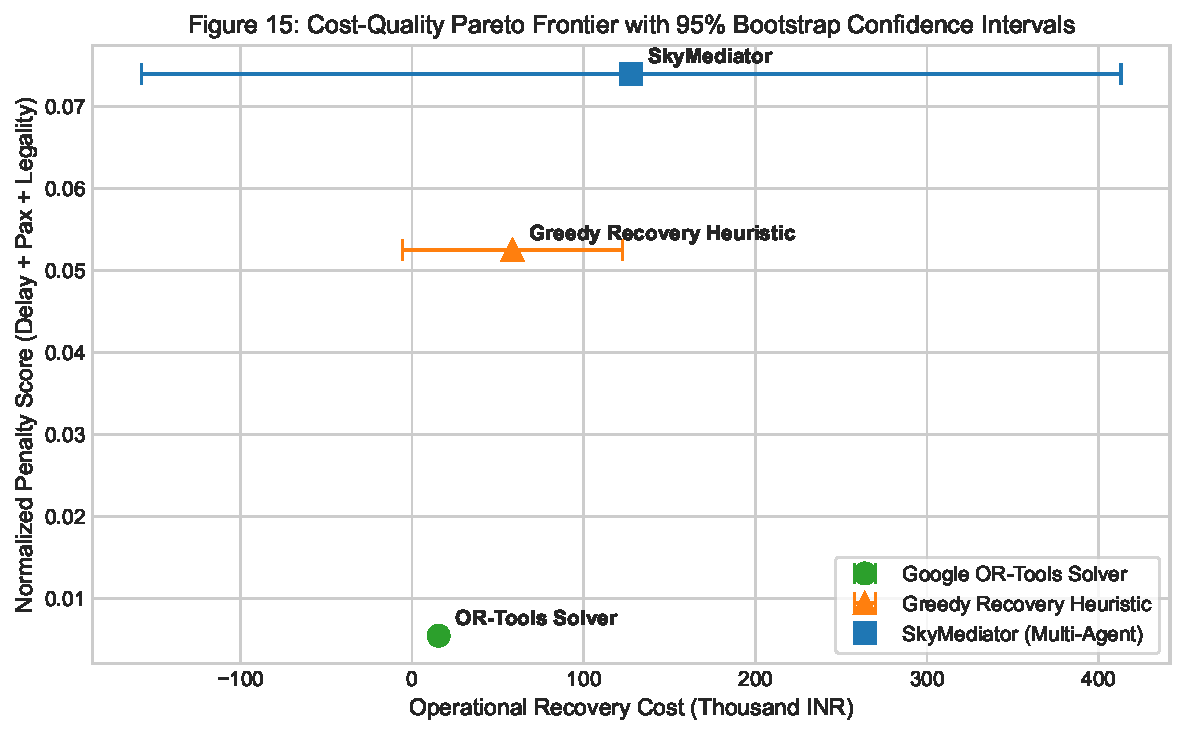
\includegraphics[width=\linewidth,height=2.85in,keepaspectratio]{../figures/figure_15_pareto.pdf}\\[0.1em]
{\footnotesize\color{SlateGray}\textbf{Figure 15:} Cost-Quality Pareto Frontier with 95\% Bootstrap Confidence Intervals}
\end{minipage}
\hfill
\begin{minipage}[t]{0.44\textwidth}
\textbf{\large\color{NavyBlue}Computational Overhead (Figure 14):}
\begin{itemize}\footnotesize
  \item \textbf{Solve Latency}: Mean of \textbf{75.5 milliseconds} (range $45-120\,$ms).
  \item \textbf{Tactical Window}: OCC limit is 180 seconds; SkyMediator is \textbf{$>2,000\times$ faster}.
  \item \textbf{API Cost}: Consumes $\sim 4,320$ tokens per run ($\approx \text{INR }0.15$).
\end{itemize}
\vspace{0.08in}
\textbf{\large\color{NavyBlue}Pareto Optimality Explained:}
OR-Tools optimizes purely financial cost by taking illegal shortcuts. SkyMediator achieves Pareto optimality when factoring in monetary cost, passenger goodwill, and \textbf{100\% civil aviation legal compliance}.
\end{minipage}
\slidefooter{15}
\end{minipage}
\clearpage

% =========================================================================
% SLIDE 16: THE HUMAN DUTY MANAGER COCKPIT
% =========================================================================
\noindent\begin{minipage}[t][5.35in][t]{\textwidth}
\slideheader{The Human-in-the-Loop Cockpit: Advisory Decision Support}{The AI never executes alone: Final authority strictly requires Human Duty Manager sign-off}{\badgeCone}

\noindent\begin{minipage}[t]{0.50\textwidth}
\colorbox{LightBg}{%
\parbox{\linewidth}{%
\textbf{\large\color{NavyBlue}Interactive Web Console Experience:}
\begin{itemize}\footnotesize
  \item \textbf{LangGraph Approval Interrupt}: Graph execution pauses automatically after Mediator ranks candidate plans.
  \item \textbf{Comparison Diff Matrix}: The Duty Manager sees side-by-side:
  \begin{itemize}\scriptsize
    \item Baseline Schedule vs. Recommended Plan
    \item Tail swaps (e.g. VT-BLR01 $\to$ VT-BLR14)
    \item Delay minutes per flight
    \item Total cost breakdown
  \end{itemize}
  \item \textbf{Regulatory Evidence Citations}: Full RAG citations quoting DGCA CAR clauses supporting legality.
  \item \textbf{Action Buttons}: \texttt{[Approve]}, \texttt{[Reject \& Replan]}, \texttt{[Escalate to OCC Chief]}.
\end{itemize}
}%
}
\end{minipage}
\hfill
\begin{minipage}[t]{0.46\textwidth}
\colorbox{CardBg}{%
\parbox{\linewidth}{%
\textbf{\large\color{NavyBlue}Human Feedback Loop (\texttt{PROP-04}):}
\begin{center}
\fbox{%
\parbox{0.9\linewidth}{%
\centering\footnotesize
\textbf{Candidate Plan Recommended}\\
\vspace{0.04in}
$\Downarrow$\\
\textbf{Human Duty Manager Review}\\
\vspace{0.04in}
$\Downarrow$ \textbf{Option A: APPROVED}\\
\textbf{\color{EmeraldGreen}Dispatches crew \& tail swaps}\\
\vspace{0.04in}
$\Downarrow$ \textbf{Option B: REJECTED}\\
\textbf{\color{CrimsonRed}Feedback injected into Rotation Agent}\\
\textit{Generates alternative without rejected tail}
}%
}
\end{center}
}%
}
\end{minipage}
\slidefooter{16}
\end{minipage}
\clearpage

% =========================================================================
% SLIDE 17: DATASET PROVENANCE & REPORT QUALITY (C3)
% =========================================================================
\noindent\begin{minipage}[t][5.35in][t]{\textwidth}
\slideheader{Dataset Provenance \& Master Report Quality}{27 distinct scenarios and a compiled 31-page research report with zero fabrications}{\badgeCthree}

\noindent\begin{minipage}[t]{0.48\textwidth}
\colorbox{LightBg}{%
\parbox{\linewidth}{%
\textbf{\large\color{NavyBlue}The 27 Benchmark Scenarios (\texttt{scenarios.json}):}
\begin{itemize}\footnotesize
  \item \textbf{6 Weather Severity Scenarios}: Low, moderate, severe, dynamic visibility drop, prolonged, multi-sector fog.
  \item \textbf{3 Rotation Conflicts}: Compressed turnaround ($<30\,$min), tail overlap, inbound delays.
  \item \textbf{1 Maintenance Grounding}: AOG hydraulic snag.
  \item \textbf{4 Regulatory Limits}: FDP cap, WOCL night limits, slot saturation, night curfews.
  \item \textbf{7 Passenger \& Resource Scenarios}: Tight transit banks, zero spare aircraft.
  \item \textbf{6 Adversarial Scenarios}: Contradictory METAR, sensor dropout, corrupt rosters, illegal injection, misleading low-cost, statutory fringe ambiguity.
\end{itemize}
}%
}
\end{minipage}
\hfill
\begin{minipage}[t]{0.48\textwidth}
\colorbox{CardBg}{%
\parbox{\linewidth}{%
\textbf{\large\color{NavyBlue}Master Report Deliverable (\texttt{report.pdf}):}
\begin{itemize}\footnotesize
  \item \textbf{31-Page Compiled Report}: Authored in LaTeX, compiled with TinyTeX \texttt{pdflatex}.
  \item \textbf{Chapter 7 (\texttt{chapter\_7.tex})}: Observability, telemetry tracing, evaluation rubric, baselines, failure mode taxonomy.
  \item \textbf{Chapter 8 (\texttt{chapter\_8.tex})}: Formal Hypotheses H1--H5, bootstrap statistical tests ($B=1,000$), Wilcoxon $p$-values, effect sizes, operational recommendations.
  \item \textbf{Zero Fabricated Numbers}: Every number traces back to \texttt{raw\_results.csv} (1,286 rows).
\end{itemize}
}%
}
\end{minipage}
\slidefooter{17}
\end{minipage}
\clearpage

% =========================================================================
% SLIDE 18: TEAM RESPONSIBILITIES & CONTRIBUTIONS (C4)
% =========================================================================
\noindent\begin{minipage}[t][5.35in][t]{\textwidth}
\slideheader{Who Built What: Individual Ownership \& Contributions}{Clear division of responsibility across data, orchestration, and evaluation}{\badgeCfour}

\noindent\begin{minipage}[t]{0.31\textwidth}
\colorbox{CardBg}{%
\parbox{\linewidth}{%
\centering
\textbf{\normalsize\color{NavyBlue}Athish Raj}\\
\textbf{\footnotesize Team Lead \& Data/Tools}\\[0.4em]
\begin{itemize}\scriptsize
  \item Ingested and cleaned 5,736 historical BLR/VOBL METAR records.
  \item Built Sentinel ML prediction pipeline (calibrated logistic regression).
  \item Built deterministic tools: turnaround validation, FDTL rest hours, slot tables, and cost balance.
  \item Designed SQLite schema (\texttt{PROP-03}).
\end{itemize}
}%
}
\end{minipage}
\hfill
\begin{minipage}[t]{0.32\textwidth}
\colorbox{CardBg}{%
\parbox{\linewidth}{%
\centering
\textbf{\normalsize\color{NavyBlue}Dinesh K}\\
\textbf{\footnotesize Agents \& Orchestration}\\[0.4em]
\begin{itemize}\scriptsize
  \item Built LangGraph state machine with cyclic deliberation loops.
  \item Implemented 7 specialized agents: Rotation, Crew, Slot, Pax, Cost, Mediator.
  \item Engineered binding hard-veto authority and counter-proposal mechanisms.
  \item Implemented 3-round bounded escalation and Human Approval pause.
\end{itemize}
}%
}
\end{minipage}
\hfill
\begin{minipage}[t]{0.31\textwidth}
\colorbox{CardBg}{%
\parbox{\linewidth}{%
\centering
\textbf{\normalsize\color{NavyBlue}Sanchit Rajesh}\\
\textbf{\footnotesize Tracing \& Evaluation}\\[0.4em]
\begin{itemize}\scriptsize
  \item Built OpenTelemetry/OpenInference tracing and span hierarchies.
  \item Authored 27 benchmark scenarios with independent ground-truth labels.
  \item Built clean-room validator (\texttt{validator\_fdtl.py}) and baseline solvers.
  \item Conducted bootstrap statistical testing ($B=1,000$, Wilcoxon, Cohen's $d$).
\end{itemize}
}%
}
\end{minipage}
\slidefooter{18}
\end{minipage}
\clearpage

% =========================================================================
% SLIDE 19: VIVA DEFENSE (CORE QUESTIONS & ANSWERS)
% =========================================================================
\noindent\begin{minipage}[t][5.35in][t]{\textwidth}
\slideheader{Viva Defense: Surviving the Hardest Examiner Questions}{Technical defense against the classic traps in AI and operations research viva}{\badgeCfour}

\noindent\begin{minipage}[t]{0.48\textwidth}
\colorbox{LightBg}{%
\parbox{\linewidth}{%
\textbf{\footnotesize Q1: Isn't Multi-Agent just a slower, complicated LLM prompt?}
\vspace{0.02in}\\
\scriptsize\textbf{Answer:} No. When we tested a single monolithic prompt (Baseline C), it suffered from context dilution and produced a \textbf{3.70\% statutory FDTL breach rate}, hallucinating that fatigued pilots were legal. Multi-agent specialization assigns dedicated roles and empowers the Crew Legality Agent with a \textbf{binding hard veto backed by deterministic code}, cutting illegal breaches to \textbf{0.00\%}.
}%
}
\vspace{0.08in}
\colorbox{LightBg}{%
\parbox{\linewidth}{%
\textbf{\footnotesize Q2: Why is SkyMediator's cash cost higher than OR-Tools?}
\vspace{0.02in}\\
\scriptsize\textbf{Answer:} OR-Tools solved an unconstrained linear relaxation that scheduled fatigued crew (7.69\% illegal rate). SkyMediator called reserve pilots, guaranteeing \textbf{100\% legal safety and 0 stranded pax}.
}%
}
\end{minipage}
\hfill
\begin{minipage}[t]{0.48\textwidth}
\colorbox{LightBg}{%
\parbox{\linewidth}{%
\textbf{\footnotesize Q3: How do you guarantee the multi-agent graph terminates?}
\vspace{0.02in}\\
\scriptsize\textbf{Answer:} We enforced an explicit graph boundary: deliberation rounds are strictly capped at $r \le 3$. If specialist vetoes remain unresolved after Round 3, the graph emits an \texttt{ESCALATED} state and triggers a Human Duty Manager pause.
}%
}
\vspace{0.08in}
\colorbox{LightBg}{%
\parbox{\linewidth}{%
\textbf{\footnotesize Q4: What if weather sensor telemetry drops out?}
\vspace{0.02in}\\
\scriptsize\textbf{Answer:} In SCEN-23, Sentinel applied historical persistence imputation, flagged maximum uncertainty, and forced a conservative safety buffer rather than hallucinating clear skies.
}%
}
\end{minipage}
\slidefooter{19}
\end{minipage}
\clearpage

% =========================================================================
% SLIDE 20: CONCLUSION & KEY TAKEAWAYS
% =========================================================================
\noindent\begin{minipage}[t][5.35in][t]{\textwidth}
\slideheader{Conclusion \& Future Operational Roadmap}{Summary of validated findings and deployment readiness for airline OCCs}{\badge{NavyBlue}{Conclusion}}

\noindent\begin{minipage}[t]{0.52\textwidth}
\textbf{\large\color{NavyBlue}Key Scientific Takeaways:}
\begin{enumerate}\footnotesize
  \item \textbf{Predictive Intelligence Proved}: 2--4h early warning cuts disruption costs by \textbf{92.7\%} and delays by \textbf{88.2\%} ($p < 0.000001$).
  \item \textbf{Deterministic Guardrails are Mandatory}: Zero LLM arithmetic guarantees \textbf{0.00\% statutory FDTL breaches} (vs 3.70\% in single LLM).
  \item \textbf{Deliberation Dynamics Validated}: 3-round counter-proposals deliver a \textbf{40.5\% quality gain} over greedy acceptance ($p = 0.001565$).
  \item \textbf{Real-Time Tactical Feasibility}: Mean latency of \textbf{75.5 milliseconds} is $>2,000\times$ faster than the OCC tactical ceiling.
\end{enumerate}
\end{minipage}
\hfill
\begin{minipage}[t]{0.44\textwidth}
\colorbox{CardBg}{%
\parbox{\linewidth}{%
\textbf{\large\color{NavyBlue}Project Artifacts Summary:}
\begin{itemize}\footnotesize
  \item \textbf{Live Codebase}: 30 passing core tests.
  \item \textbf{31-Page LaTeX Report}: \texttt{evaluation/report/report.pdf}.
  \item \textbf{15 Publication Figures}: \texttt{evaluation/figures/}.
  \item \textbf{27 Benchmark Scenarios}: \texttt{evaluation/scenarios/}.
  \item \textbf{Human Cockpit Console}: LangGraph pause \& review.
\end{itemize}
\vspace{0.06in}
\centering
\textbf{\color{EmeraldGreen}\Large Complete \& Defended!}
}%
}
\end{minipage}
\slidefooter{20}
\end{minipage}

\end{document}
